% $HeadURL$

\subsection{Glyph: \glyph{Simple chemical}}
\label{sec:simpleChemical}

A simple chemical in SBGN is defined as the opposite of a macromolecule (\sect{macromolecule}): it is a chemical compound that is \emph{not} formed by the covalent linking of pseudo-identical residues.  Examples of simple chemicals are an atom, a monoatomic ion, a salt, a radical, a solid metal, a crystal, etc.

\begin{glyphDescription}

\glyphSboTerm SBO:0000247 ! simple chemical

\glyphContainer A \glyph{simple chemical} is represented by a circular
container, as depicted in \fig{simpleChemical}. To avoid confusion
with the Unspecified Entity (\ref{sec:unspecifiedEntity}), this glyph
must remain a circle and cannot be deformed into an eclipse.

\glyphLabel The identification of the \glyph{simple chemical} is carried by an unbordered box containing a string of characters.  The characters may be distributed on several lines to improve readability, although this is not mandatory.  The label box has to be attached to the center of the circular container.  The label is permitted to spill outside the container.

\glyphAux A \glyph{simple chemical} may be decorated with one or more \glyph{units of information} (\sect{unitInfo}).  A particular \glyph{unit of information} describes the material type.  A \glyph{simple chemical} may also carry a \glyph{clone marker} (\sect{cloneMarker}).

\end{glyphDescription}

\begin{figure}[H]
  \centering
  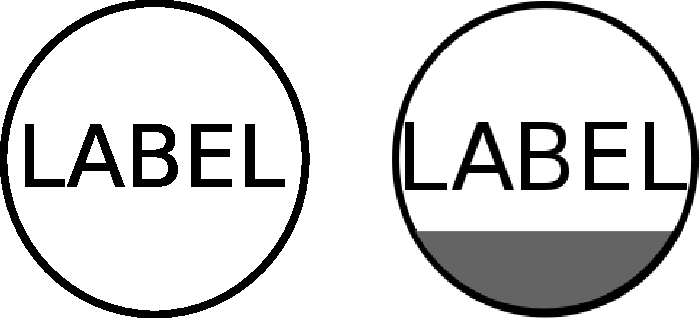
\includegraphics[scale = 0.3]{images/simpleChemical}
  \caption{The \PD glyph for \glyph{simple chemical}.}
  \label{fig:simpleChemical}
\end{figure}

% The following is for [X]Emacs users.  Please leave in place.
% Local Variables:
% TeX-master: "../sbgn_PD-level1"
% End:
